% Definiciones y constantes de estilo
% Clase del documento
\documentclass[a4paper,12pt,twoside,openright,titlepage]{book}

%
% Paquetes necesarios
%

% Codificación UTF8
\usepackage[utf8]{inputenc}
% Title
\usepackage{titling}
% Márgenes
\usepackage[hmargin=3cm,vmargin=3.5cm]{geometry}
% Definición de colores
\usepackage{color}
% Extensión del paquete color
\usepackage[table,xcdraw,dvipsnames]{xcolor}
% Cabecera y pie de página
\usepackage{fancyhdr}
% Estilo título capítulos
\usepackage{quotchap}
% Títulos de secciones
\usepackage{titlesec}
% Enumeraciones
\usepackage{enumerate}
% Páginas en blanco
\usepackage{emptypage}
% Código, algoritmos, etc.
\usepackage{listings}
% Separación entre cajas
\usepackage{float}
% Imágenes
\usepackage[pdftex]{graphicx}
% Incluir pdfs externos
\usepackage{pdfpages}
% Apéndices
\usepackage{appendix}
% Marcadores (para el pdf)
\usepackage{bookmark}
% Estilo de enumeraciones
\usepackage{enumitem}
% Espacio entre líneas y párrafos
\usepackage{setspace}
% Glosario/Acrónimos
\usepackage[acronym]{glossaries}
% Fuentes
\usepackage[T1]{fontenc}
% Tables
\usepackage{tabularx}
\usepackage{longtable}

% Subtitle
\newcommand{\subtitle}[1]{%
	\posttitle{%
		\par\end{center}
		\begin{center}\large#1\end{center}
		\vskip0.5em
		}%
}

% Enlaces
\hypersetup{
	hidelinks,
	pageanchor=true,
	colorlinks,
	citecolor=Fuchsia,
	urlcolor=blue,
	linkcolor=black
}
\urlstyle{same}

% Euro (€)
\DeclareUnicodeCharacter{20AC}{\euro}

% Inclusión de gráficos
\graphicspath{{./images/}}

% Extensiones de gráficos
\DeclareGraphicsExtensions{.pdf,.jpeg,.jpg,.png}

% Definiciones de colores (para hidelinks)
\definecolor{LightCyan}{rgb}{0,0,0}
\definecolor{Cerulean}{rgb}{0,0,0}
\definecolor{Fuchsia}{rgb}{0,0,0}

% Estilo páginas de capítulos
\fancypagestyle{plain}{
\fancyhf{}
\fancyfoot[CO]{\thepage}
\renewcommand{\footrulewidth}{.6pt}
\renewcommand{\headrulewidth}{0.0pt}
}

% Estilo resto de páginas
\pagestyle{fancy}

\renewcommand\thesection{\arabic{section}}

% Guía del pie de página
\renewcommand{\footrulewidth}{.6pt}

% Nombre del titulo para indice de codigo
\renewcommand\lstlistlistingname{Table of code}

% Nombre de los bloques de código
\renewcommand{\lstlistingname}{Code}

% Estilo de los lstlistings
\lstset{
    frame=tb,
    breaklines=true,
    showstringspaces=false,
    postbreak=\raisebox{0ex}[0ex][0ex]{\ensuremath{\color{gray}\hookrightarrow\space}}
}

% Definiciones de funciones para los títulos
\newlength\salto
\setlength{\salto}{3.5ex plus 1ex minus .2ex}
\newlength\resalto
\setlength{\resalto}{2.3ex plus.2ex}

% Estilo de los acrónimos
\renewcommand{\acronymname}{Acronym}
\renewcommand{\glossaryname}{Acronym}
\pretolerance=2000
\tolerance=3000

% Comando code (lstlisting sin cambio de página)
\lstnewenvironment{code}[1][]%
  { \noindent\minipage{0.935\linewidth}\medskip
    \vspace{5mm}
    \lstset{basicstyle=\ttfamily\footnotesize,#1}}
  {\endminipage}

% Numerado hasta sub subsecciones
\setcounter{secnumdepth}{3}

\title{Big Data:\\ Design of a new interactive data analysis tool}
\subtitle{Máster Universitario en Ingeniería Informática\\
		  Universidad Politécnica de Madrid}
\author{Group 22:\\
		José Domínguez Pérez\\
		Ismael Muñoz Aztout\\
		Jonatan Ruedas Mora}
\date{January 2021}

\makeindex
\begin{document}
\maketitle
\tableofcontents
\newpage

\section{Introduction}

We have selected a dataset based on films due the fact that we really love films and we think that the topic could be quite interesting, specially if we are able to show the evolution of the film industry in the last decades.

We have chosen \href{https://www.kaggle.com/tmdb/tmdb-movie-metadata?select=tmdb_5000_movies.csv}{The Movie Database dataset} in order to carry out our practical work.

\subsection{Dataset description}
Our dataset consists of table with items and attributes. More specifically, it is a Flat Table with an explicit index (ID) of categorical type. 

\begin{center}
\begin{longtable}[c]{| c | c | c |}
 \hline
 \multicolumn{1}{| c |}{\bfseries Variable} & \multicolumn{1}{| c |}{\bfseries Type} & \multicolumn{1}{| c |}{\bfseries Description}\\
 \hline
 \endfirsthead
  
 \hline
 \endhead
 
 \hline
 \endfoot  
 
 \hline
 \endlastfoot  
  
 Budget & Integer & Budget of the movie  \\
  \hline
 Genres & JSON & Genres of the movie  \\
  \hline
 Keywords  & JSON  & Keywords related to the movie  \\
  \hline
 Production$\textunderscore$companies & JSON & Companies that produced the movie  \\
  \hline
 Revenue  & Integer  & Revenue of the movie  \\
  \hline
 Runtime  & Integer  & Duration of the movie in minutes  \\
  \hline
 Vote$\textunderscore$average  & Integer  & Rating of the movie given by the users  \\
  \hline
 Tittle  & String  & Name of the movie  \\
  \hline
 Release$\textunderscore$date  & Date  & Release date of the movie  \\
  \hline
 Production$\textunderscore$countries  & JSON  & Countries that have produced the movie  \\
  \hline
 Homepage  & String  & Webpage of the movie  \\
  \hline
 Id  & Integer  & Movie identifier  \\
  \hline
 Original$\textunderscore$language  & String  & Original language of the movie  \\
  \hline
 Original$\textunderscore$title  & String  & Original title of the movie  \\
  \hline
 Overview  & String  & Description of the movie  \\
  \hline
 Popularity  & Integer  & Popularity of the movie  \\
  \hline
 Spoken$\textunderscore$languages  & JSON  & Different spoken languages in the movie  \\
  \hline
 Status  & String  & Status of the movie  \\
  \hline
 Tagline  & String  & Brief description of the movie  \\
  \hline
 Vote$\textunderscore$count  & Integer  & Number of votes that the movie has received  \\
\hline
\end{longtable}
\end{center}

The columns that we use are:

\begin{center}
\begin{longtable}[c]{| c | c | c |}
 \hline
 \multicolumn{1}{| c |}{\bfseries Variable} & \multicolumn{1}{| c |}{\bfseries Type} & \multicolumn{1}{| c |}{\bfseries Description}\\
 \hline
 \endfirsthead
  
 \hline
 \endhead
 
 \hline
 \endfoot  
 
 \hline
 \endlastfoot
 
 Budget  & Integer  & Budget of the movie  \\
  \hline
 Genres  & JSON  & Genres of the movie  \\
  \hline
 Keywords  & JSON  & Keywords related to the movie  \\
  \hline
 Production$\textunderscore$companies & JSON & Companies that produced the movie  \\
  \hline
 Revenue  & Integer  & Revenue of the movie  \\
  \hline
 Vote$\textunderscore$average  & Integer  & Rating of the movie given by the users  \\
  \hline
 Release$\textunderscore$date  & Date  & Release date of the movie  \\
  \hline
 Production$\textunderscore$countries  & JSON  & Countries that have produced the movie  \\
\hline
\end{longtable}
\end{center}

The columns that we have produced are:

\begin{center}
\begin{longtable}[c]{| c | c | c |}
 \hline
 \multicolumn{1}{| c |}{\bfseries Variable} & \multicolumn{1}{| c |}{\bfseries Type} & \multicolumn{1}{| c |}{\bfseries Description}\\
 \hline
 \endfirsthead
  
 \hline
 \endhead
 
 \hline
 \endfoot  
 
 \hline
 \endlastfoot  
 
 Year  & Integer  & Year of the release  \\
  \hline
 Month  & Integer  & Month of the release  \\
  \hline
 Day  & Integer  & Day of the release  \\
  \hline
 Decade  & Integer  & Decade of the release  \\
  \hline
 Earnings  & Integer  & Earnings of a movie  \\
\hline
\end{longtable}
\end{center}

We had to parse the columns that contain JSON values to String in order to have a better structure to be able to retrieve the required information.

\section{Problem characterization}

The domain in which we have worked on is the one related to the movie industry, so terms like budget, revenue, ratings are used everywhere. This domain does not have many fuzzy words, as a consequence, it has been quite easy to understand its vocabulary.\\

Apart from that, as we do not have access to experts in the topic, we have tried put ourselves into a movie analyst shoes, in order to think what kind of questions we would want to explain to the public to ilustrate how the industry has evolved over the last 50 years.\\

The questions that we have raised for this practical work are the following:

\begin{enumerate}
	\item When is more profitable to release a film?
	\item How the popularity of the companies has evolved over time?
	\item Which are the most remarkable genres and keywords in the movie industry of a country?
\end{enumerate}

\section{Data and Task abstractions}

\subsection{First Question}

\subsubsection{Target}
The target of this question the \textit{Period of the year in which it is more profitable to release a film}. This target can be classified as an Atribute $\,\to\,$ One $\,\to\,$ Distribution.

\subsubsection{Abstract Data}

First of all, we had to think what kind of data do we need to answer the first question properly. We realized that we need to produce some data in order to know the \textit{Decade}, \textit{Month} and the \textit{Earnings} of the different films.\\

We have decided to use the \textit{Decade} instead of the \textit{Year} because there were many years and as the film industry usually categorize films by decades we thought that it could be a good option.\\

The attributes that we use for this question are the following:

\begin{itemize}
	\item \textbf{Consumed attributes}
		\begin{itemize}
			\item \textit{Budget}: Ordered $\,\to\,$ Quantitative $\,\to\,$ Sequential.
			\item \textit{Revenue}: Ordered $\,\to\,$ Quantitative $\,\to\,$ Sequential.
			\item \textit{Release$\textunderscore$date}: Ordered $\,\to\,$ Ordinal $\,\to\,$ Secuential.
		\end{itemize}
	\item \textbf{Produced attributes} (these attributes have been produced on the EDA)
		\begin{itemize}
			\item \textit{Year}: Ordered $\,\to\,$ Ordinal $\,\to\,$ Sequential.
			\item \textit{Month}: Ordered $\,\to\,$ Ordinal $\,\to\,$ Cyclic.
			\item \textit{Decade}: Ordered $\,\to\,$ Ordinal $\,\to\,$ Sequential.
			\item \textit{Earnings}: Ordered $\,\to\,$ Quantitative $\,\to\,$ Diverging.
		\end{itemize}
\end{itemize}

\subsubsection{Abstract Tasks}

The abstract tasks that we have defined for this question are the following:

\begin{itemize}
	\item \textbf{Produce $\,\to\,$ Derive}. We combine the variables Revenue and Budget to produce the Earnings.
	\item \textbf{Consume $\,\to\,$ Discover $\,\to\,$ Generate}. We are generating an hypothesis about when is more profitable to release a movie.
	\item \textbf{Search $\,\to\,$ Explore}. We do not know the period of the year in which it is better to release a film.
	\item \textbf{Query $\,\to\,$ Identify}. We are identifying the most profitable time to release a film.
\end{itemize}

\subsection{Second Question}

\subsubsection{Target}
We have defined the next target to this question: \textit{Evolution of the popularity of the companies over the years}. The defined target can be classified as All data $\,\to\,$ Trend.

\subsubsection{Abstract Data}

In order to answer this question we realized that we will need the following data:

\begin{itemize}
	\item \textbf{Consumed attributes}
		\begin{itemize}
			\item \textit{Vote$\textunderscore$average}: Ordered $\,\to\,$ Quantitative $\,\to\,$ Sequential.
			\item \textit{Production$\textunderscore$companies}: Categorical.
			\item \textit{Year}: Ordered $\,\to\,$ Ordinal $\,\to\,$ Sequential.
		\end{itemize}
\end{itemize}

\subsubsection{Abstract Tasks}

The abstract tasks that we have defined for this question are the following:

\begin{itemize}
	\item \textbf{Consume $\,\to\,$ Present $\,\to\,$}. We want to present the evolution (trend) of the popularity of the companies over time. We already have this data so we do not need to generate more data..
	\item \textbf{Search $\,\to\,$ Explore}. We do not know the evolution of the popularity of the companies and we do not know where to search for it.
	\item \textbf{Query $\,\to\,$ Compare}. We want to compare the evolution of different companies
\end{itemize}

\subsection{Third Question}

\subsubsection{Target}
The target for this question is: \textit{Most remarkable genres of films and keywords of a country}. It can be classified as All data $\,\to\,$ Outliers.

\subsubsection{Abstract Data}

To tackle this question we need this data:

\begin{itemize}
	\item \textbf{Consumed attributes}
		\begin{itemize}
			\item \textit{Genres}: Categorical.
			\item \textit{Production$\textunderscore$countries}: Categorical.
		\end{itemize}
	\item \textbf{Produced attributes}
		\begin{itemize}
			\item \textit{Frequency of movies in a genre by country}: Ordered $\,\to\,$ Quantitative $\,\to\,$ Sequential.
			\item \textit{Frequency of keywords by country}: Ordered $\,\to\,$ Quantitative $\,\to\,$ Sequential.
		\end{itemize}
\end{itemize}

\subsubsection{Abstract Tasks}

We have selected the next abstract tasks for this question:

\begin{itemize}
	\item \textbf{Consume $\,\to\,$ Enjoy}. We feel curiosity to know which are the most important genres and keywords by country.
	\item \textbf{Search $\,\to\,$ Lookup}. We know the number of movies in a genre and the number of keywords by country, and also we do know where to find them.
	\item \textbf{Query $\,\to\,$ Identify}. We want to identify the outliers.
\end{itemize}

\section{Interaction and visual encoding}

\subsection{First Question}

The methods that we have selected to interact with the visualization are the following:

\begin{itemize}
	\item \textbf{Filter}: We filter by decades to reduce the size of the dataset in order to have a clear view of the data.
\end{itemize}

To encode the data we have used a Heatmap. We have selected this idiom because we have two ordered variables, \textit{Year} and \textit{Month}, that can act as categorical, and a quantitative variable, so we can use the categorical variables in the axis and let the quantitative for the cells of the heatmap.\\

The X-axis represents the years of the selected \textit{Decade} while the Y-axis encodes the different months. Finally, the cells encode the \textit{Earnings} of the movies that have been released in a specific month of a year.\\

We have used a green tone and we vary its saturation to obtain a green scale that represents the \textit{Earnings}.\\

The figure \ref{fig:1st_question} ilustrates the idiom that we have selected.

\begin{figure}[H]
	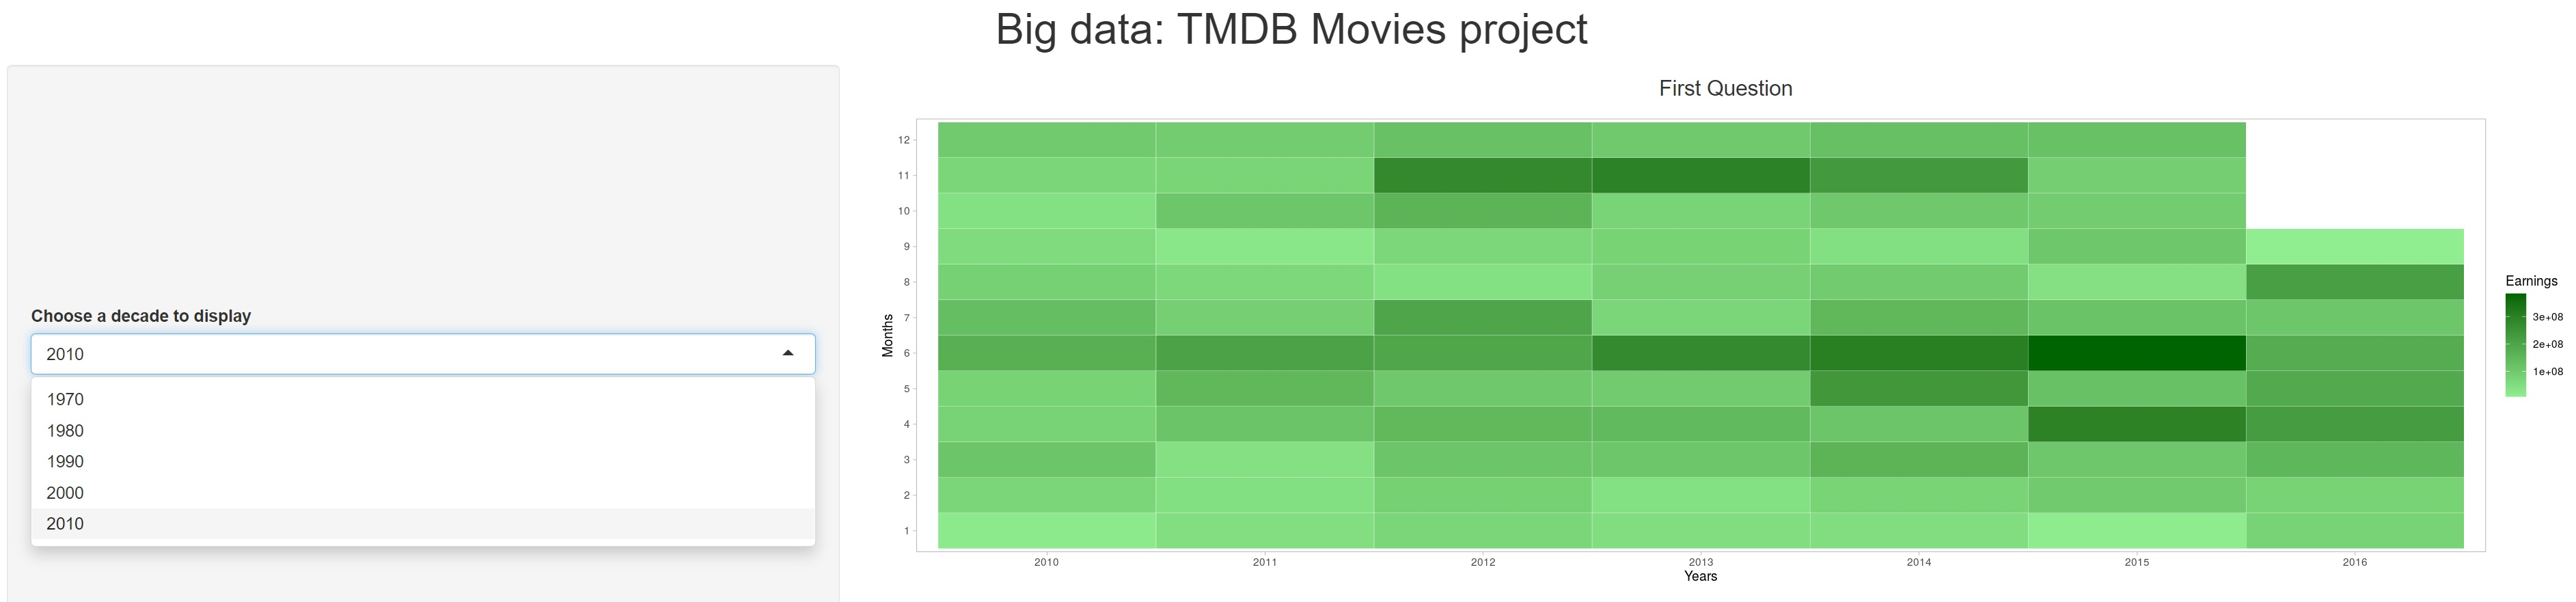
\includegraphics[scale=.3]{question_1}
	\caption{First question: 2010 decade}
	\label{fig:1st_question}
\end{figure}

\subsection{Second Question}

We have selected the following methods to interact with the visualization:

\begin{itemize}
	\item \textbf{Filter}: We filter can filter by a group of years.
	\item \textbf{Facet $\,\to\,$ Superimpose}: We overlap the evolution of different companies in the same visualization.
\end{itemize}

In order to encode the data we have selected a Line chart because these plots are perfect to show changes over certain periods of time. In our case, these changes will be the variation of the average rating and we will be able to overlap different companies to compare them.\\

The X-axis represents the \textit{years} that the user have selected, the Y-axis shows the \textit{average rating} of a given company based on the ratings of their movies. Apart from that, every \textit{country} has a different color to improve the visual perception.\\

We only allow to compare 5 companies at the same time because because there are too much data and it wont be understandable. In addition, we do not allow to select the same year as starting and ending year with that we can assure that the minimum evolution that can be displayed is a 1 year evolution. \\

The images \ref{fig:2nd_question} and \ref{fig:2nd_question_2} shows an example of the idiom.

\begin{figure}[H]
	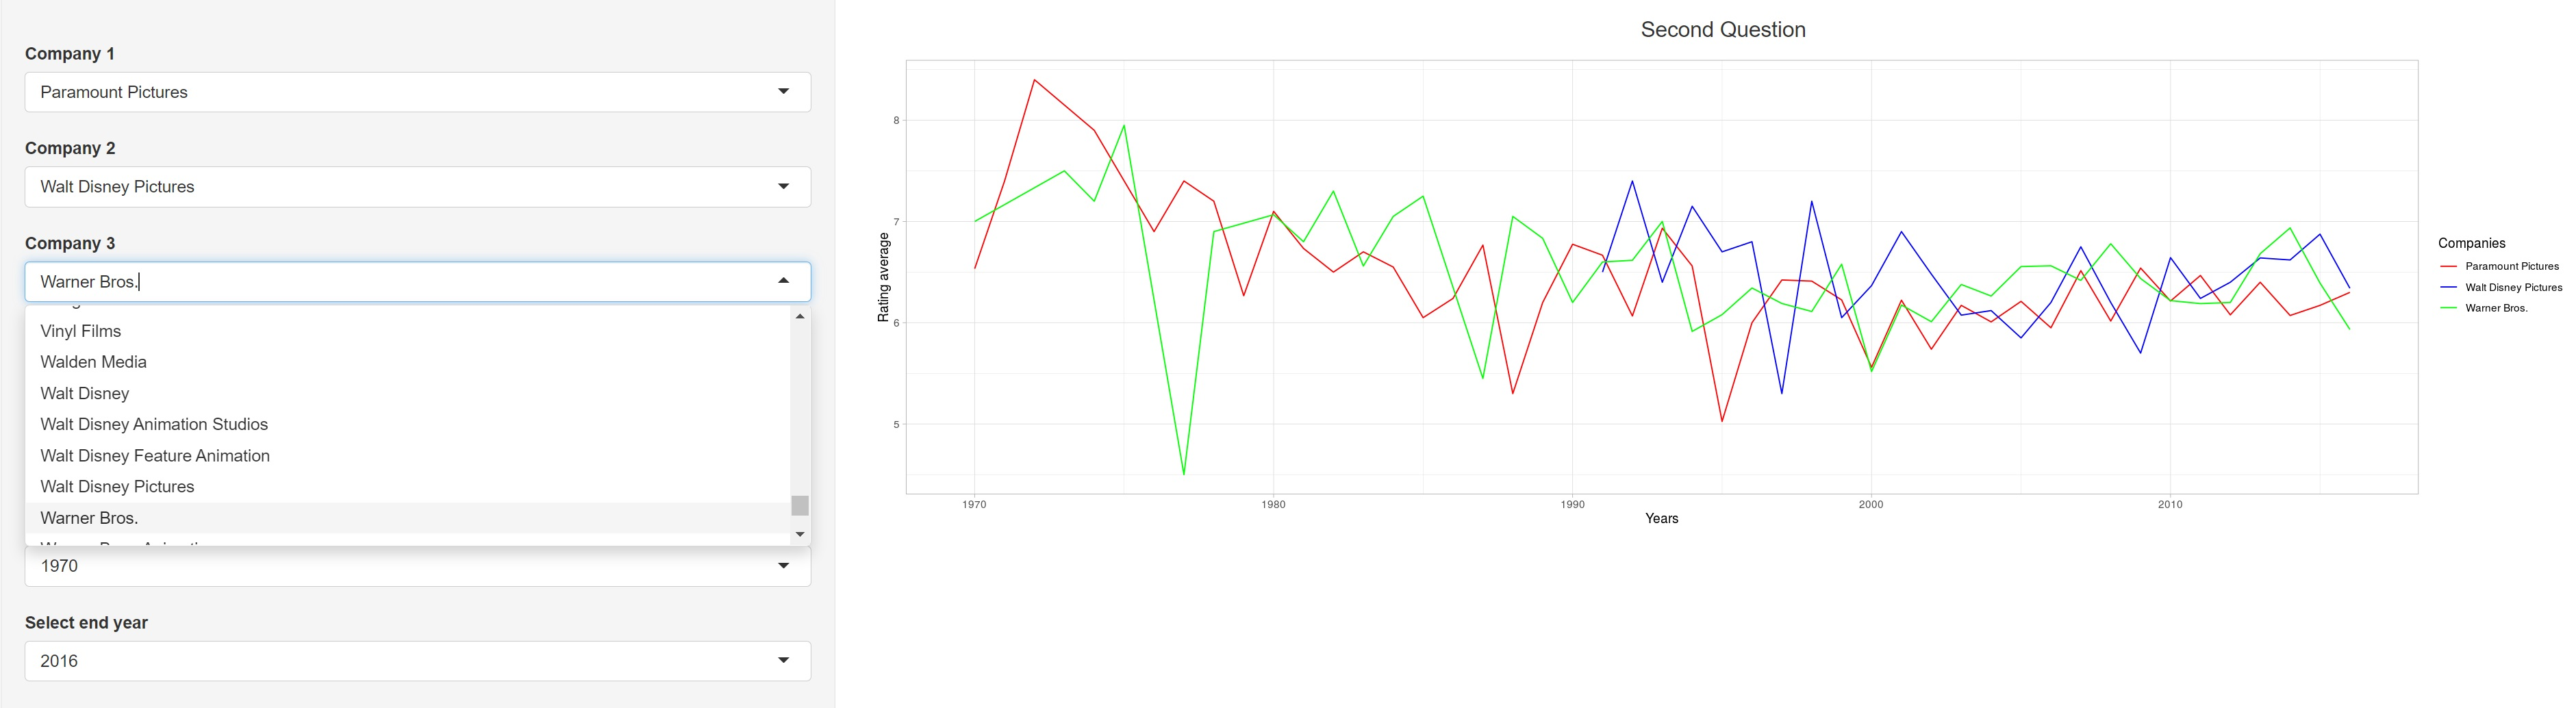
\includegraphics[scale=.3]{question_2}
	\caption{Second question: Default companies: 1970-2016}
	\label{fig:2nd_question}
\end{figure}

\begin{figure}[H]
	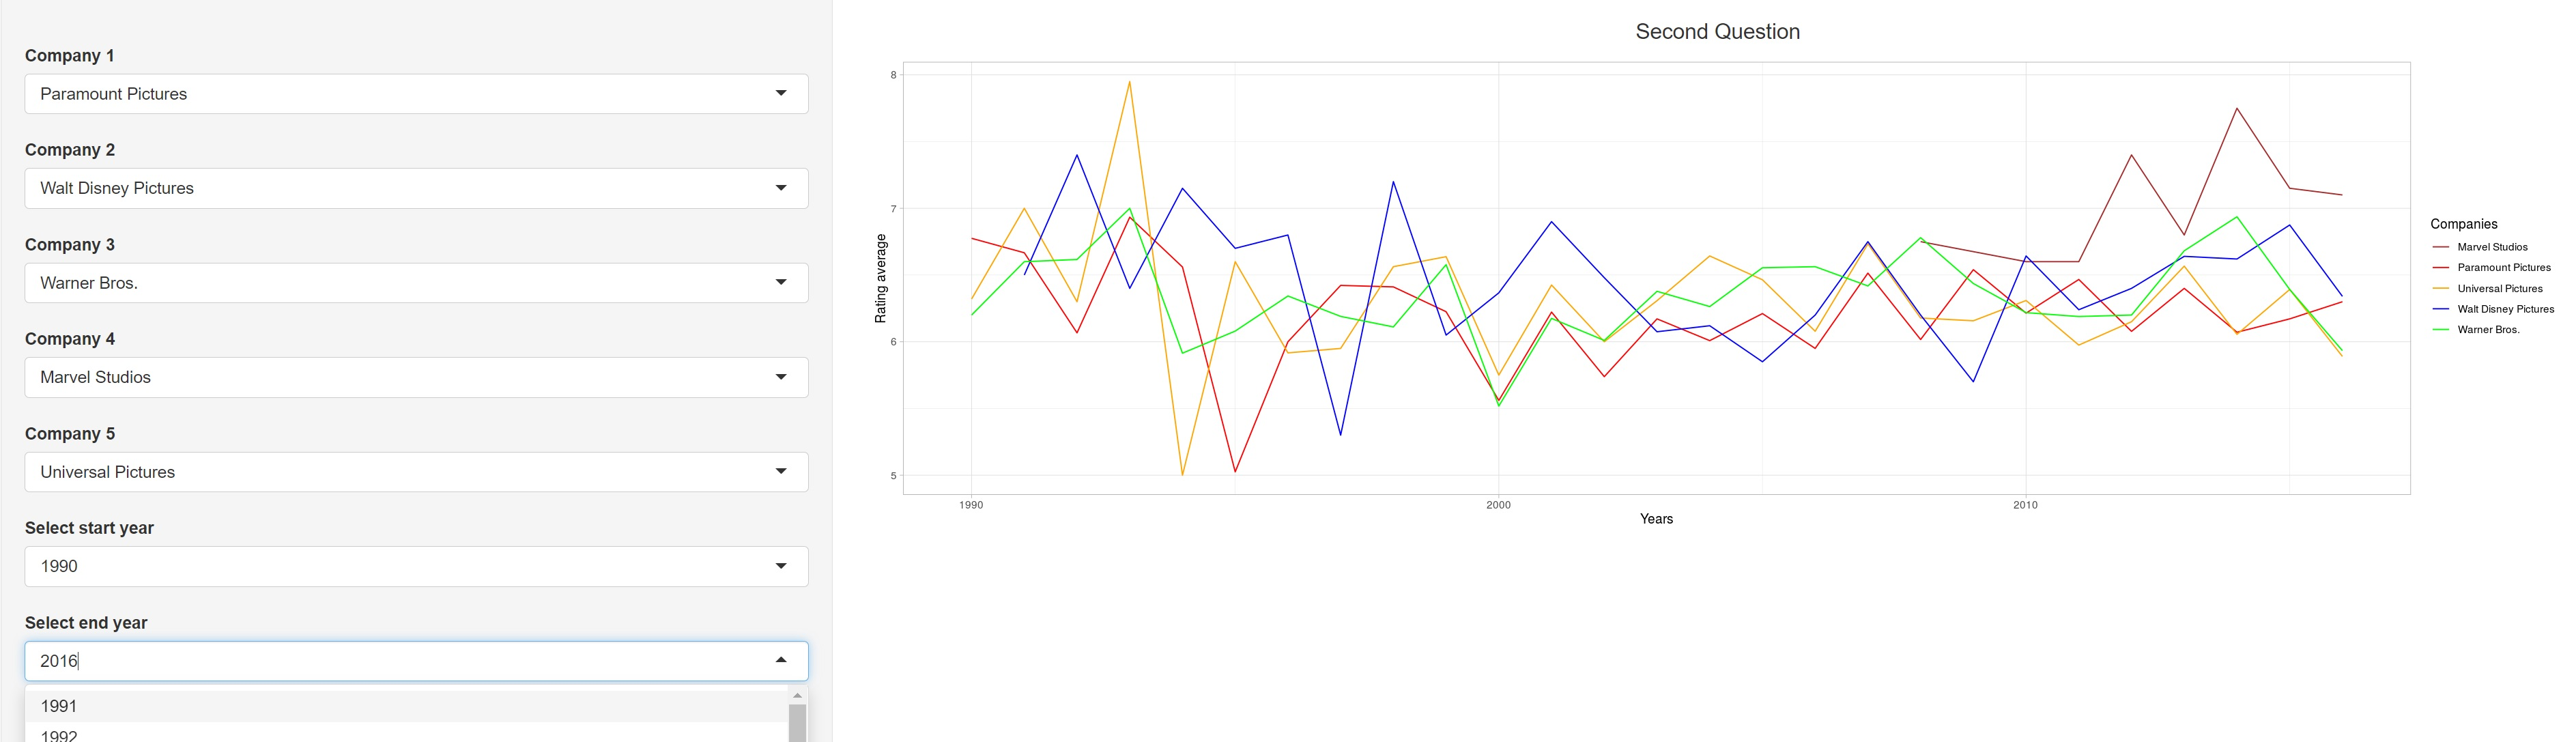
\includegraphics[scale=.3]{question_2_1}
	\caption{Second question: Maximum companies. 1988-2016}
	\label{fig:2nd_question_2}
\end{figure}

\subsection{Third Question}

The interaction with the visualization will be carried out by the following methods:

\begin{itemize}
	\item \textbf{Order}: We can order by frequency.
	\item \textbf{Filter}: We filter the data by country and by the number of keywords.
	\item \textbf{Juxtapose}: We have 2 graphics that interact at the same time when the country is selected.
\end{itemize}

A lollipop chart and a word cloud has been selected for the encoding. The first one encodes the prevalent genres in a country and the second one the most frequent keywords in a country.\\

The X-axis of the Lollipop chart encodes the \textit{Frequency} while the Y-axis encodes the \textit{Genre}.\\

We consider that both graphics are suitable to show the frequency of the data.\\

It is believed that choosing the Word Cloud is not a good decision because the area is a poor metaphor and the longer words appear bigger. We agree with those arguments, however, as we are not interested in the specific value of the frequency, we think that it could be a right choice because it highlights the most important keywords.\\

In addition, we have set a max number of characters for the keywords to avoid the problem related with the long strings mentioned before.\\

Apart from that, we allow the user to select the number of words that he wants to display. However, we have set a range for the number of words displayed in the word cloud, the minimum is 10 and the maximum is 50. \\

The figures \ref{fig:3rd_question}, \ref{fig:3rd_question_1}, \ref{fig:3rd_question_2}, \ref{fig:3rd_question_3} ilustrate the explanation about the idioms: 

\begin{figure}[H]
	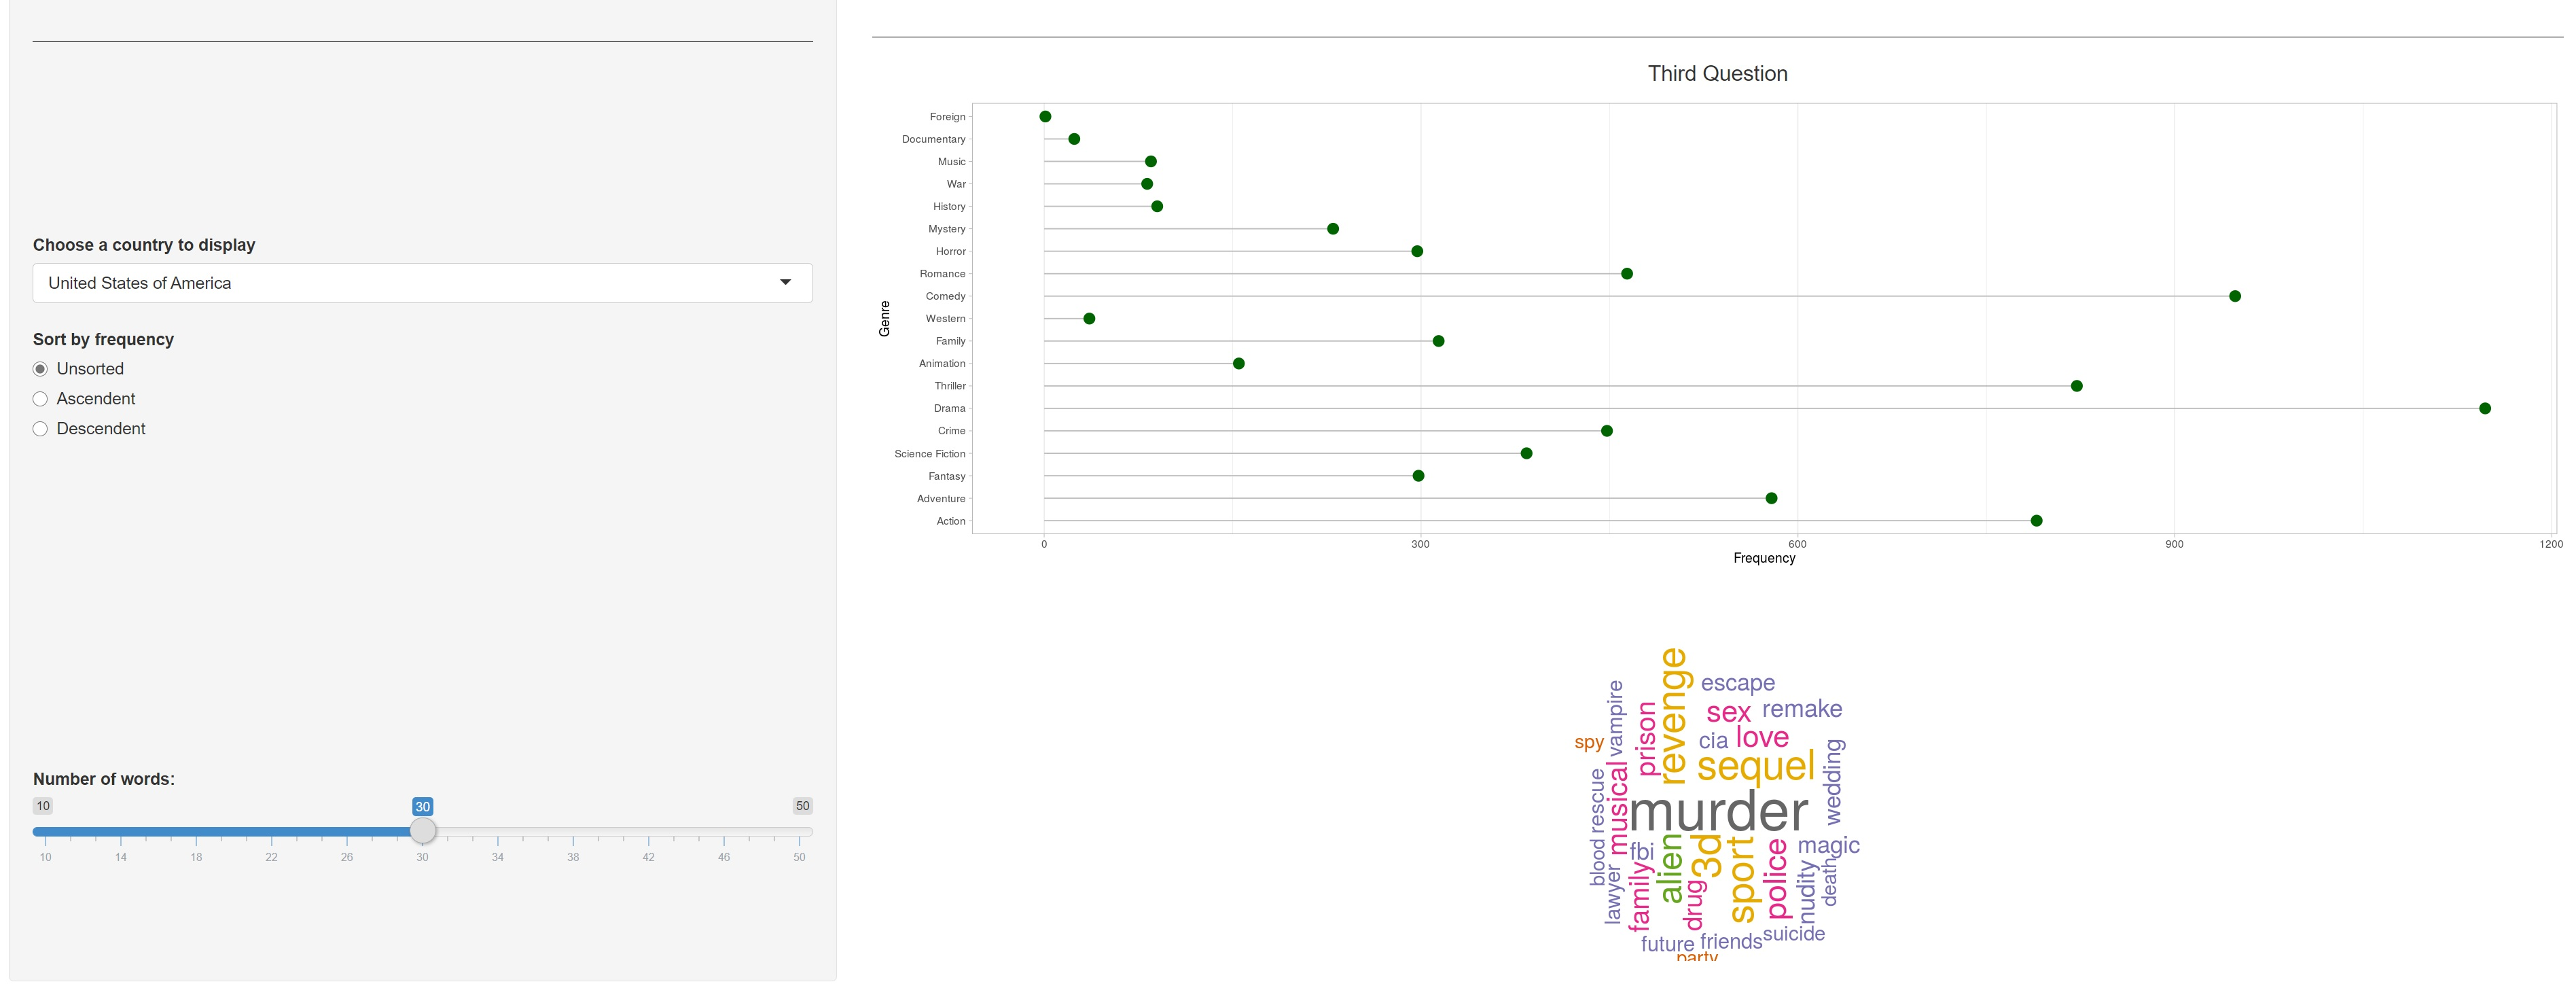
\includegraphics[scale=.3]{question_3}
	\caption{Third question: USA unsorted. 30 words. Default}
	\label{fig:3rd_question}
\end{figure}

\begin{figure}[H]
	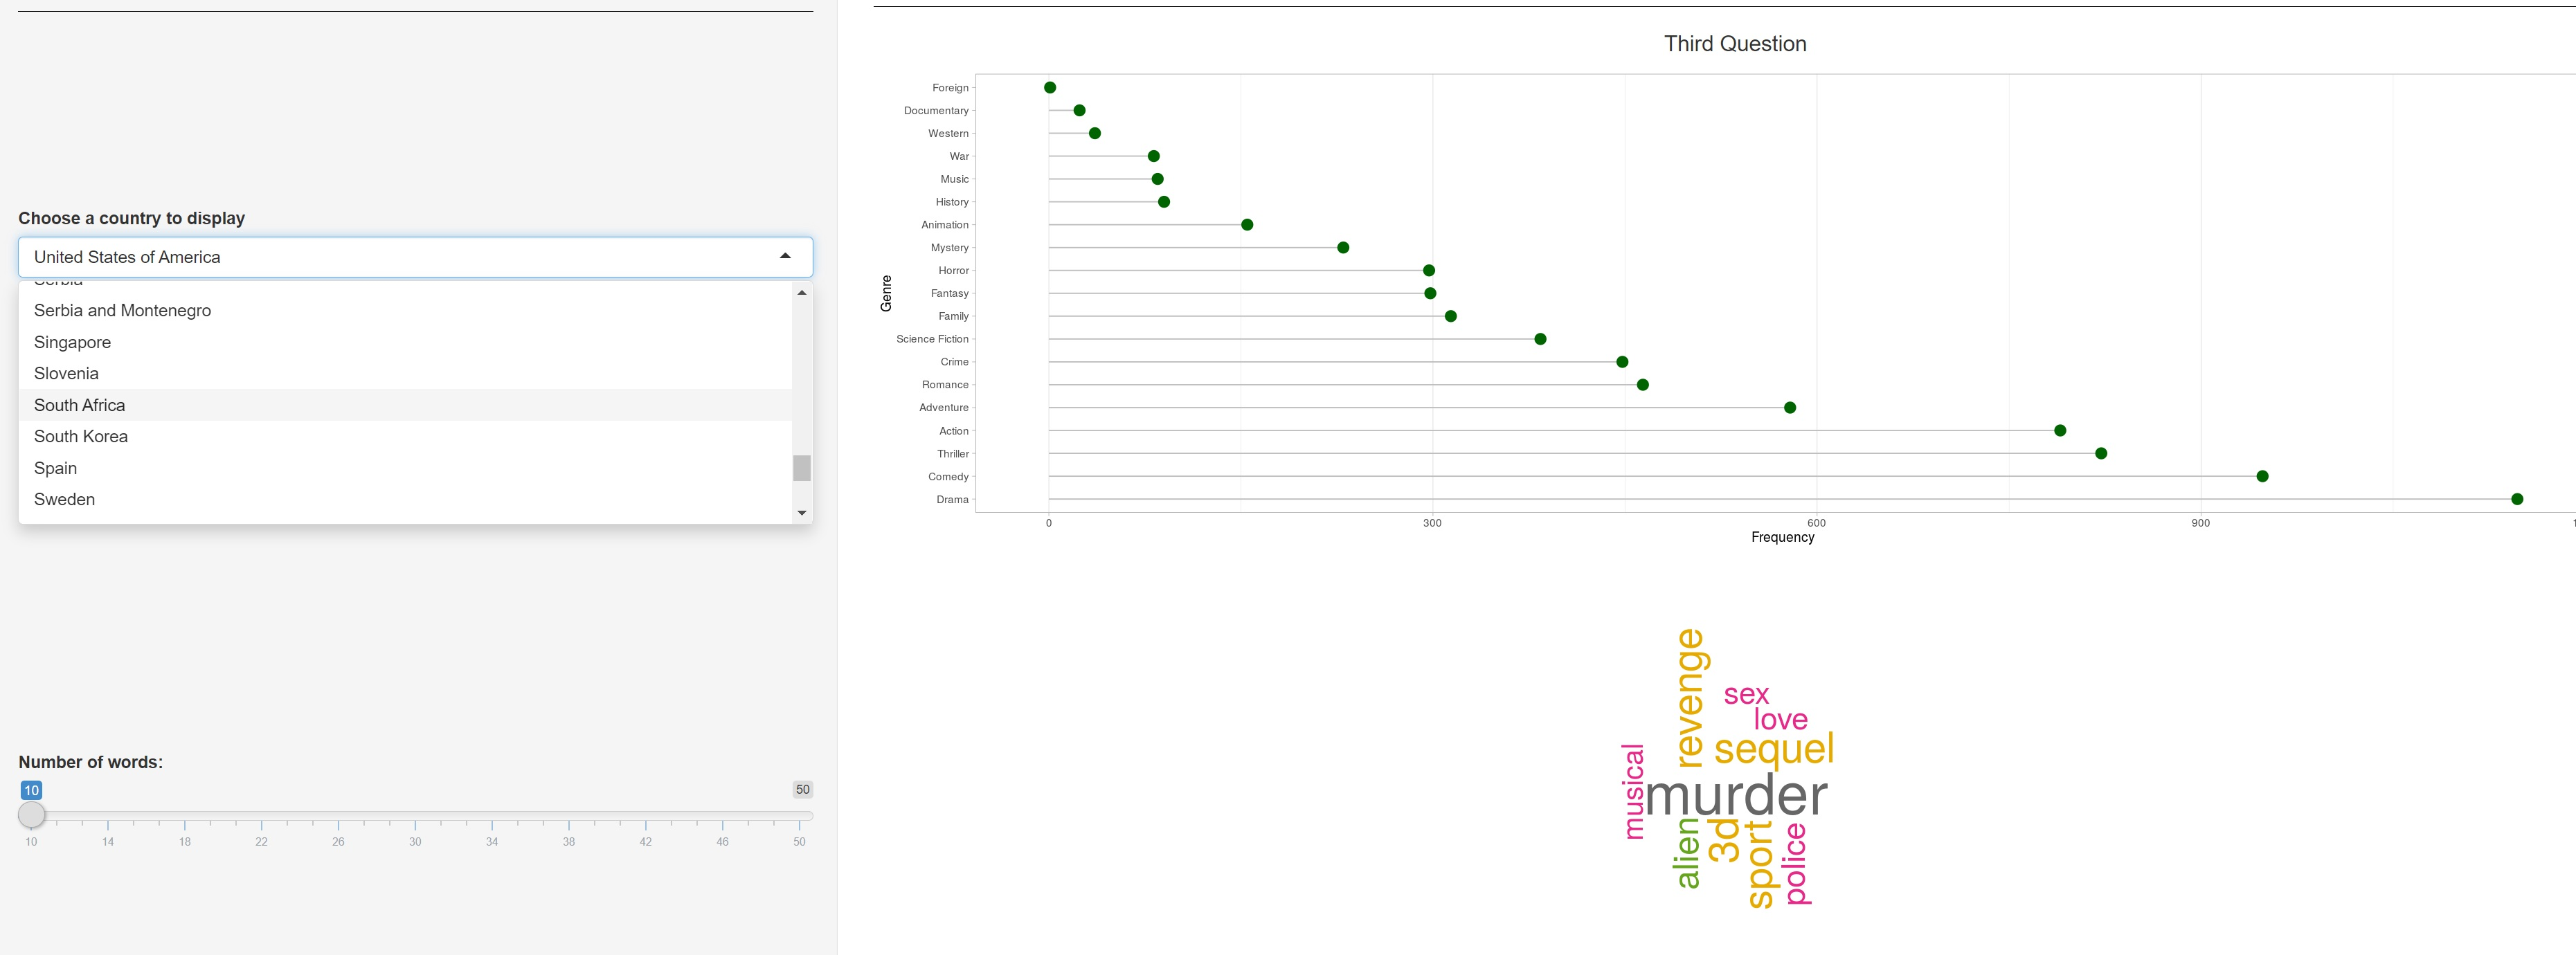
\includegraphics[scale=.3]{question_3_1}
	\caption{Third question: USA descendent. 10 words}
	\label{fig:3rd_question_1}
\end{figure}

\begin{figure}[H]
	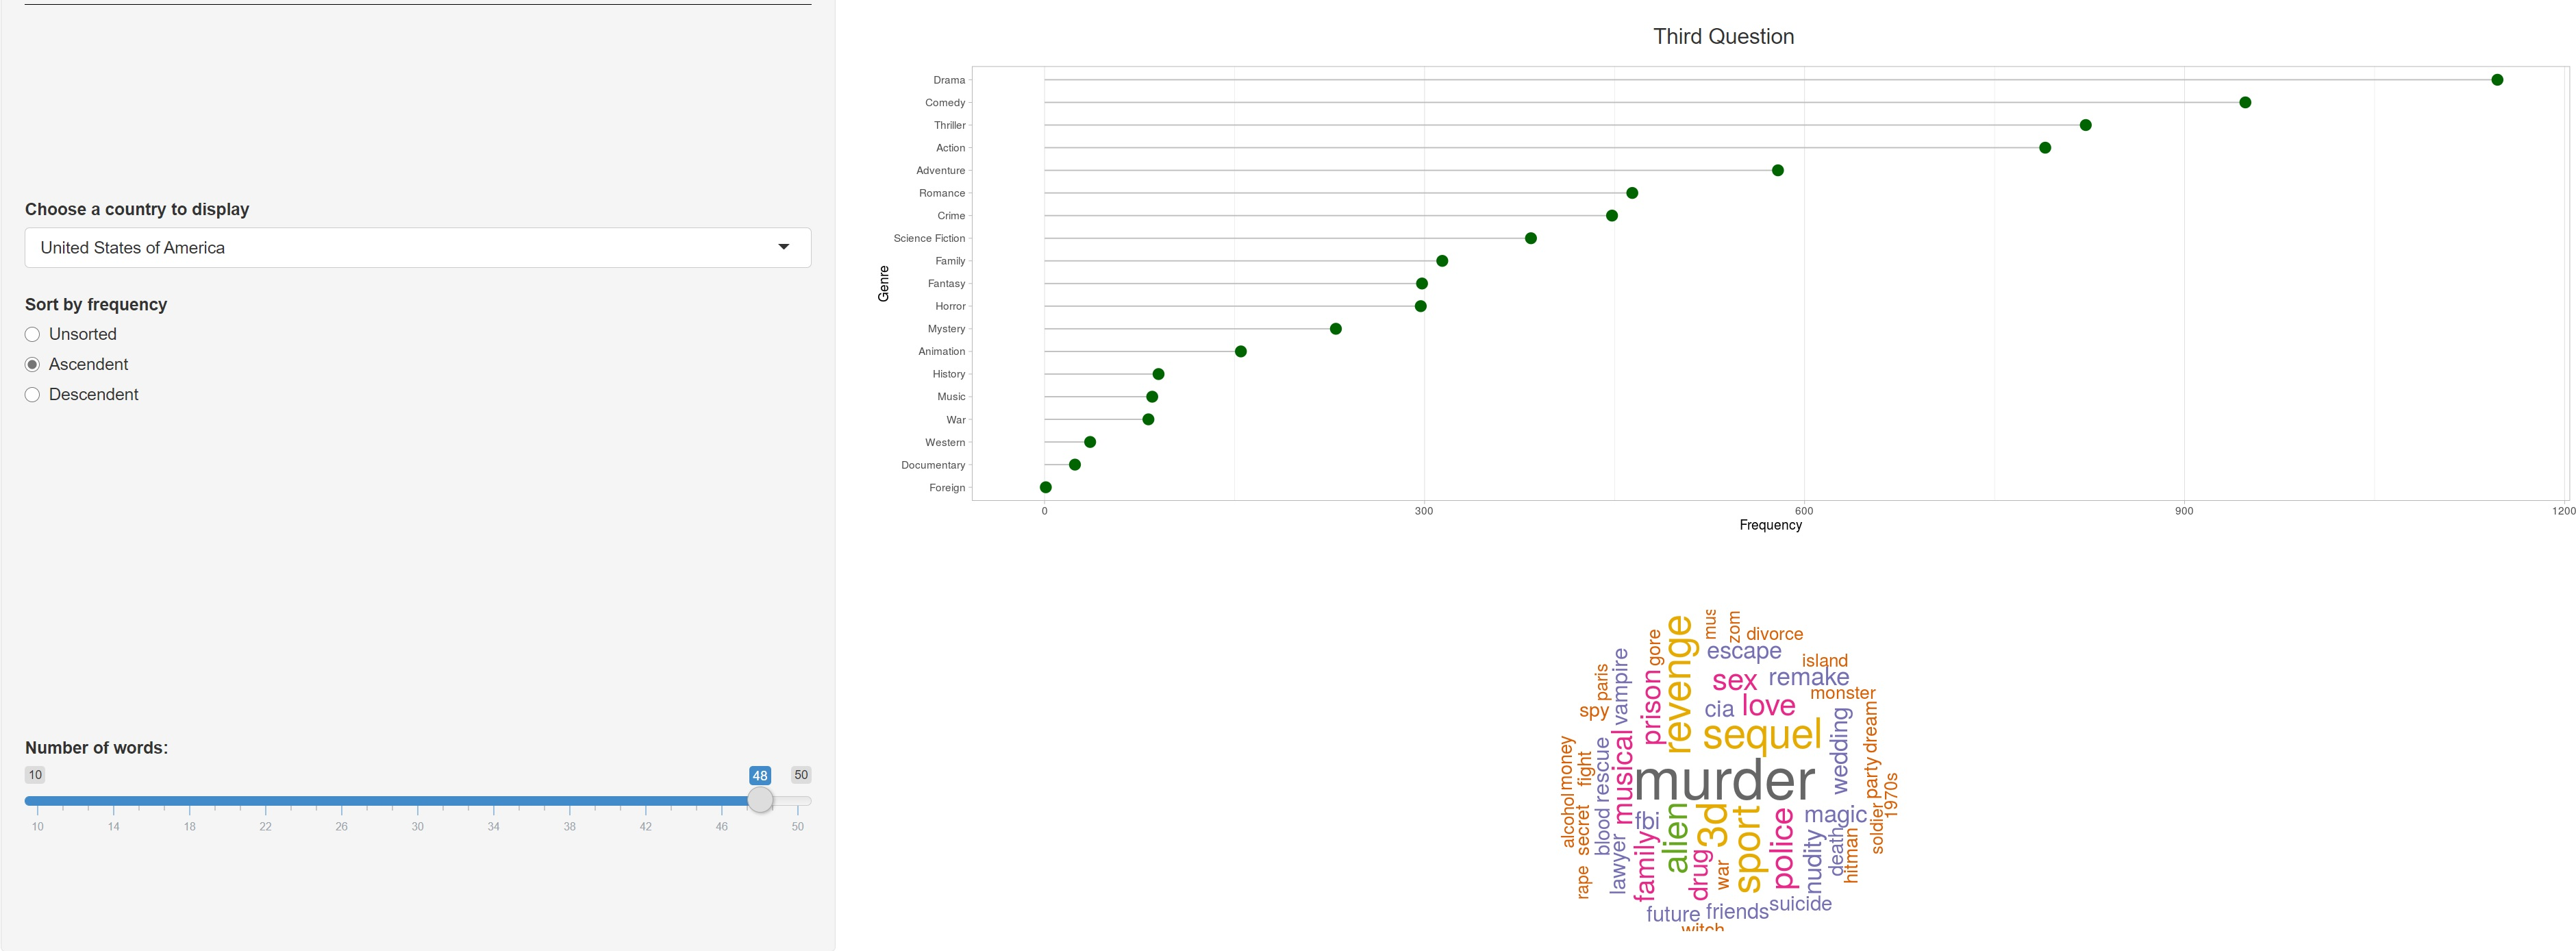
\includegraphics[scale=.3]{question_3_2}
	\caption{Third question: USA ascendent. 48 words}
	\label{fig:3rd_question_2}
\end{figure}

\begin{figure}[H]
	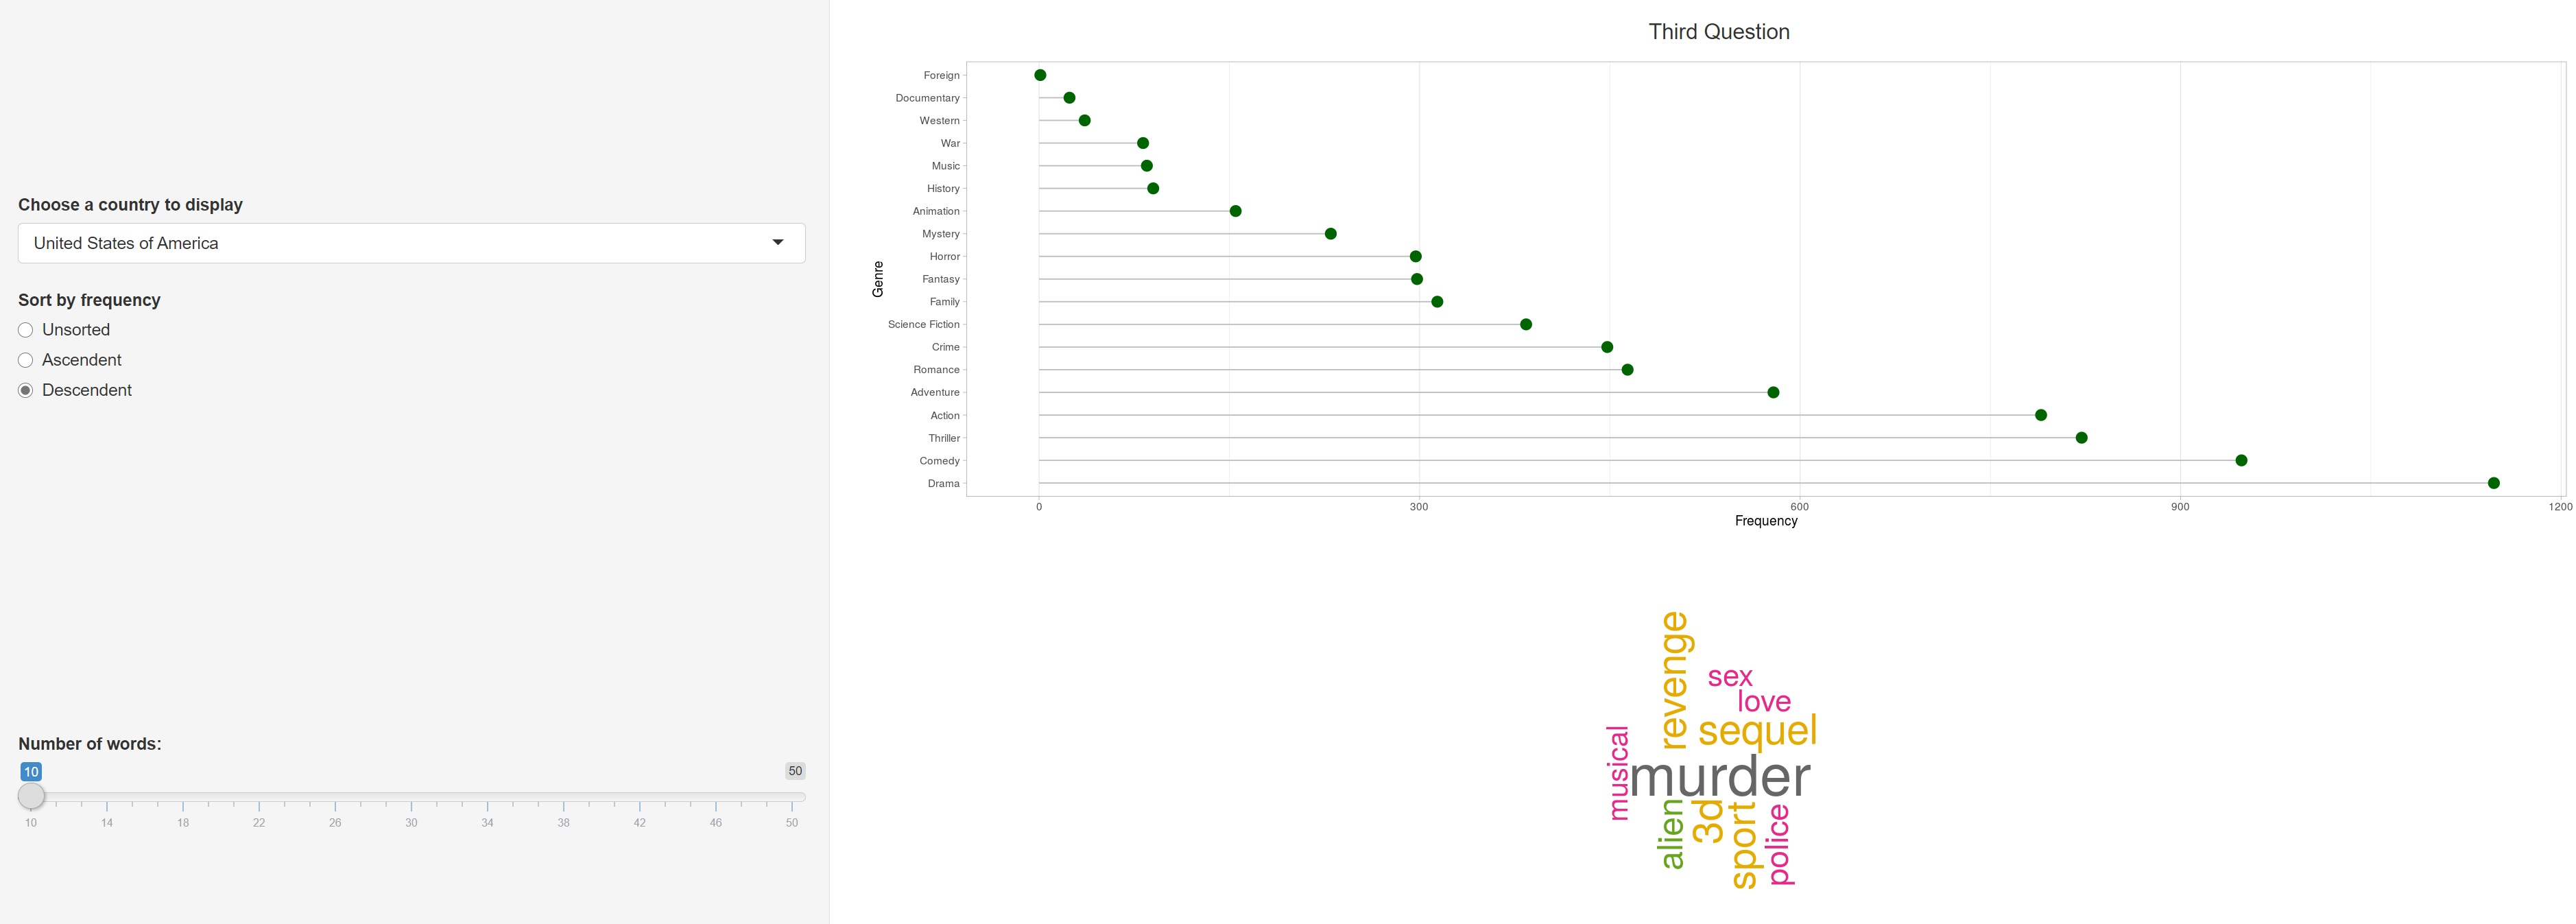
\includegraphics[scale=.3]{question_3_3}
	\caption{Third question: USA descendent. 10 words}
	\label{fig:3rd_question_3}
\end{figure}

\section{Algorithmic implementation}

Before implementing our application, we have performed a exploratory data anaylysis in order to inspect the data in more depth. Thanks to this, we have been able to realize which data is worth it and which one can be removed.\\ 

In this exploratory data analysis we have carried out the following tasks:

\begin{itemize}
	\item Keep the columns we are going to use in our application
	\item Remove missing values from the dataset
	\item Parse date to new columns
	\item Create new columns such as decade and earnings
	\item Parse JSON columns
\end{itemize}

Also, this makes the execution of our shiny app more efficient due to the fact that we simplify our dataset and the application has to deal with much less data.\\

\subsection{First Question}
In the first question, we aggregate by year and month from a selected decade and we show the result of this operation in a heatmap. In order to have the heatmap properly printed we had to factorize the years and months.

\subsection{Second Question}
In this question, we first do the following tasks outside the server function so that they are executed once in the execution of our application:

\begin{enumerate}
	\item Calculate the minimum and maximum year a company has released a film and plot the evolution of three well-known companies in this range of time by default. Then the user can select another range of years to be shown.
	\item Keep the companies that have published five or more movies in different years so that we can see an evolution in the line chart. There is no sense in making a line chart for a company that has only published very few movies as we are not going to be able to appreciate the evolution. Additionally, we remove repetitions and whitespaces that may exist.
	\item Sort the list of companies we are going to provide by name so that the user can easily identify a company. Furthermore, we add to the beginning of this list, the option to leave a company blank (choose a company). This way, the corresponding company will not be shown in the line chart. This is the default value for the fourth and fifth companies in the line chart. Then, the user can try to add more companies in order to see their evolution.
\end{enumerate}

In the server function, we associate a color with a company such that when a change in the selected companies is made, the color of the rest of the companies do not change, since this is the fault operation of the \textit{ggplot} function. In order to solve this problem, we map a color to every button in the UI, ie, the first company will be shown in red, the second one in blue, and so on. Later on, we filter the companies by the selected range of years, calculate the rating of the films of these companies between the selected range of years and plot the results in the line chart.

\subsection{Third Question}
In the third question, we first do the following tasks outside the server function so that they are only executed once in the execution of our application:

\begin{enumerate}
	\item Expanded the production countries, genres and keywords of every film as they were contained in a single cell separated by commas per every film. This way, we get a new row for every production country, genre and keyword and we can make queries to this new data. Additionally, we remove the whitespaces that may exist and the keywords that have more that seven characters so that they can be displayed properly.
	\item Gest a list of countries without repetitions to show to the user and they can select a country to be shown.
\end{enumerate}

In the server function, we do the following tasks:

\begin{enumerate}
	\item Get the frequency of the different genres of the selected country and sort the genres by name in an ascendent or descendent way if the user have selected the corresponding sorting button. By default, the genres is not sorted. Then, we display the genres and their frequency in a lollipop chart.
	\item Get the keywords related to the selected country and display them in a wordcloud allowing the user to control the number of words displayed in every moment.
\end{enumerate}
\section{Execution instructions}

\subsection{Dependencies}

The dependencies required are the following R packages:

\begin{itemize}
	\item Data exploration (\textit{dataset$\textunderscore$preparation.R}):
		\begin{itemize}
			\item \textit{rjson}
		\end{itemize}
	\item Shiny app:
		\begin{itemize}
			\item \textit{shiny}
			\item \textit{ggplot2}
			\item \textit{dplyr}
			\item \textit{tidyr}
			\item \textit{stringr}
			\item \textit{wordcloud}
		\end{itemize}
\end{itemize}

\subsection{Project structure and input data}

The app folder is called \textit{movies}.\\

Download the dataset file \textbf{tmdb$\textunderscore$5000$\textunderscore$movies.csv} from: \href{https://www.kaggle.com/tmdb/tmdb-movie-metadata?select=tmdb_5000_movies.csv}{The Movie Database dataset} and place it into the \textit{movies/data} folder. The name of the dataset file must be: \textbf{tmdb$\textunderscore$5000$\textunderscore$movies.csv}.\\

Apart from that, the \textbf{dataset$\textunderscore$preparation.R} must be executed in order to clean the data and generate the new dataset, \textbf{cleaned$\textunderscore$tmdb$\textunderscore$5000$\textunderscore$movies.csv} inside the \textit{movies/data} folder.\\

\subsection{Execution}

The Shiny app can be executed from \textit{RStudio} or from the command line interface. \\

In order to run the app from the CLI you must be in the folder that contains the \textit{movies} folder and execute the following command into an R session:

\noindent
\begin{lstlisting}[language=bash]
  $ R 
  > install.packages("shiny")
  > library(shiny)
  > runApp('movies')
\end{lstlisting}

\section{Application deployment}

The application has been deployed to \url{https://www.shinyapps.io/}. It can be found here \href{https://jruedas.shinyapps.io/movies/}{Big data: TMDB Movies project}.

\section{Final conclusions}

We found this project very interesting, we really enjoyed the R programming and Shiny. The Shiny documentation was really well written so it was easy to find out how to solve the problems. The main problem was the data preparation aspect because some columns were in JSON format so we had to parse them, and the Tasks abstractions and econding tasks, even though, this project has been educative and interesting.\\

\end{document}